\documentclass{article}
\usepackage{xeCJK}
\usepackage{amsmath}
\usepackage{graphicx}
\usepackage{algorithm}
\usepackage{algorithmic}

\setCJKmainfont{Microsoft YaHei}
\renewcommand{\algorithmicrequire}{\textbf{Input:}}
\renewcommand{\algorithmicensure}{\textbf{Output:}}
\linespread{1.5}


\begin{document}
一.
采用深度优先搜索的策略,在搜索过程中通过优先选取面值较大的硬币来决定优先搜索
对象实现搜索树剪枝。\\
具体实现中,维护一个最小堆,将$amount$减去各个面值的硬币后所剩金额压入最小堆中,
弹出顶层元素,再减去不大于其的所有面值并压入最小堆,直至顶层元素为0(或者未找到结果),
同时使用一个字典来记录硬币个数。

\begin{algorithm}
    \caption{\textbf{min\_nums}}
    \label{alg:coins}
    \begin{algorithmic}[1]
        \REQUIRE an array of coins, the total amount
        \ENSURE the min numbers used to match the amount if found, -1 if not found
        \STATE $Min\_heap\; heap$
        \STATE $Map\; path$
        \STATE $heap.push(amount)$ 
        \STATE $path.put(amount, 1)$
        \WHILE{$heap\; is\; not\; empty$}
        \STATE $top = heap.pop()$
        \STATE $len = path.get(top)$
        \IF{$top == 0$}
        \RETURN $len$
        \ENDIF
        \IF{$top < min(coins)$}
        \STATE $continue$
        \ENDIF
        \FOR{$coin\; in\; coins$}
        \IF{$top - coin \geq 0$}
        \STATE $heap.push(top - coin)$
        \STATE $path.put(top - coin, len + 1)$
        \ENDIF
        \ENDFOR
        \ENDWHILE
        \RETURN \textbf{-1}
    \end{algorithmic}
\end{algorithm}
\newpage

二:\\
(1)\\
$g(n)$ 为从起点到节点 $n$ 的代价。\\
$h*(n)$ 为从节点 $n$ 回到起点(不经过已经走过的节点)的优化路径代价。\\
(2)\\
记 \\
$h(1) = 0$, \\
$h(2) = 2$, \\
$h(3) = 3$, \\
$h(4) = 6$. \\
搜索树如下所示:\\
\begin{figure}[htbp]
    \centering
    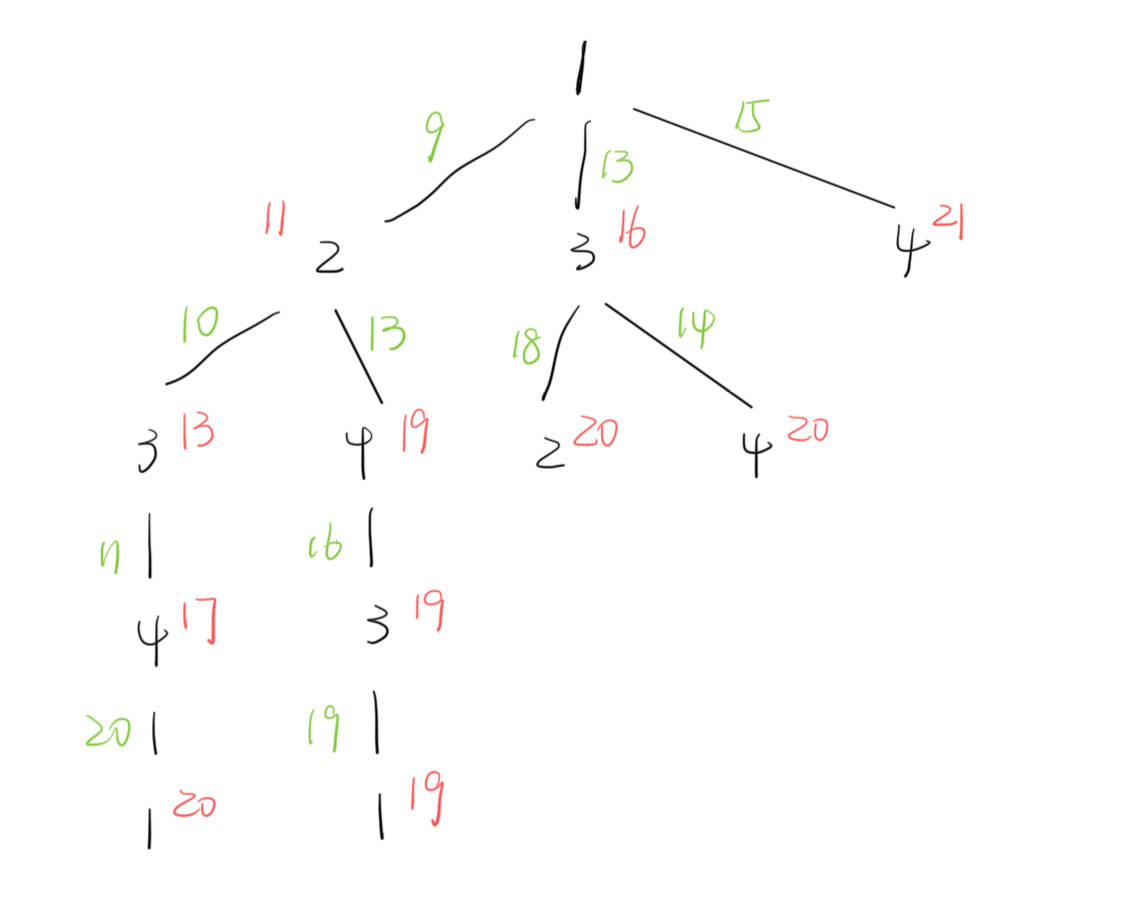
\includegraphics[width=0.5\textwidth]{2.png}
    \caption{serch tree}
\end{figure} 

\end{document}